\subsection{Plotting a discrete response: the \macro{LOGODDS}}\label{sec:logist-logodds}

It is sometimes difficult to understand how a binary response can give
rise to a smooth, continuous relationship between the predicted response
and an explanatory variable, particularly when the predictor is
continuous.
Thus, in \figref{fig:logist1c1} you can see the (0/1) responses
and the fitted relation, but it takes some effort to see that
the observation points determine that relation.
Another problem is that the age variable is not strictly continuous ---
it was recorded in whole years --- so there may be considerable
overplotting of the observation points in such a graph.

%% two subfig side-by-side
\begin{figure}[htb]
 \begin{minipage}[t]{.49\linewidth}
  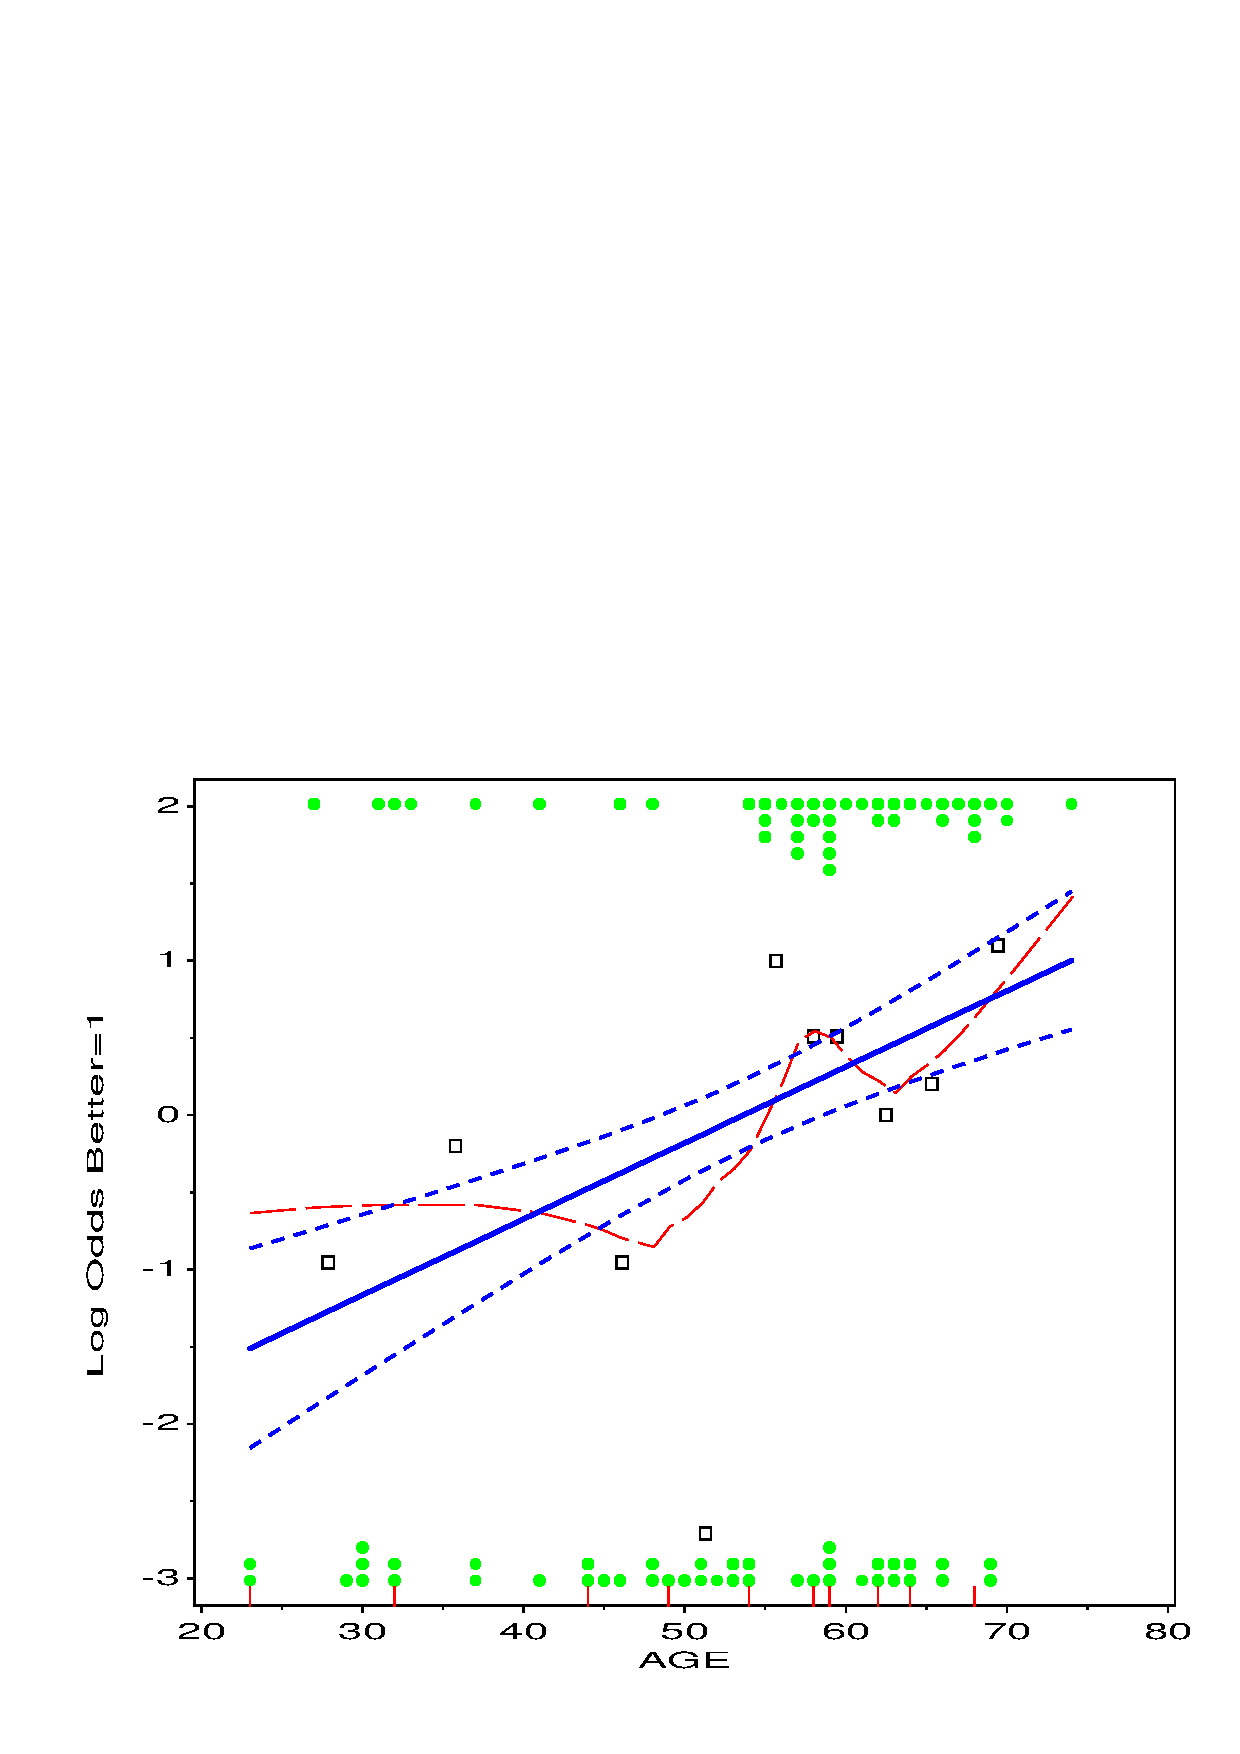
\includegraphics[width=1\linewidth]{ch6/fig/logoddt1}
 \end{minipage}%
 \hfill
 \begin{minipage}[t]{.49\linewidth}
  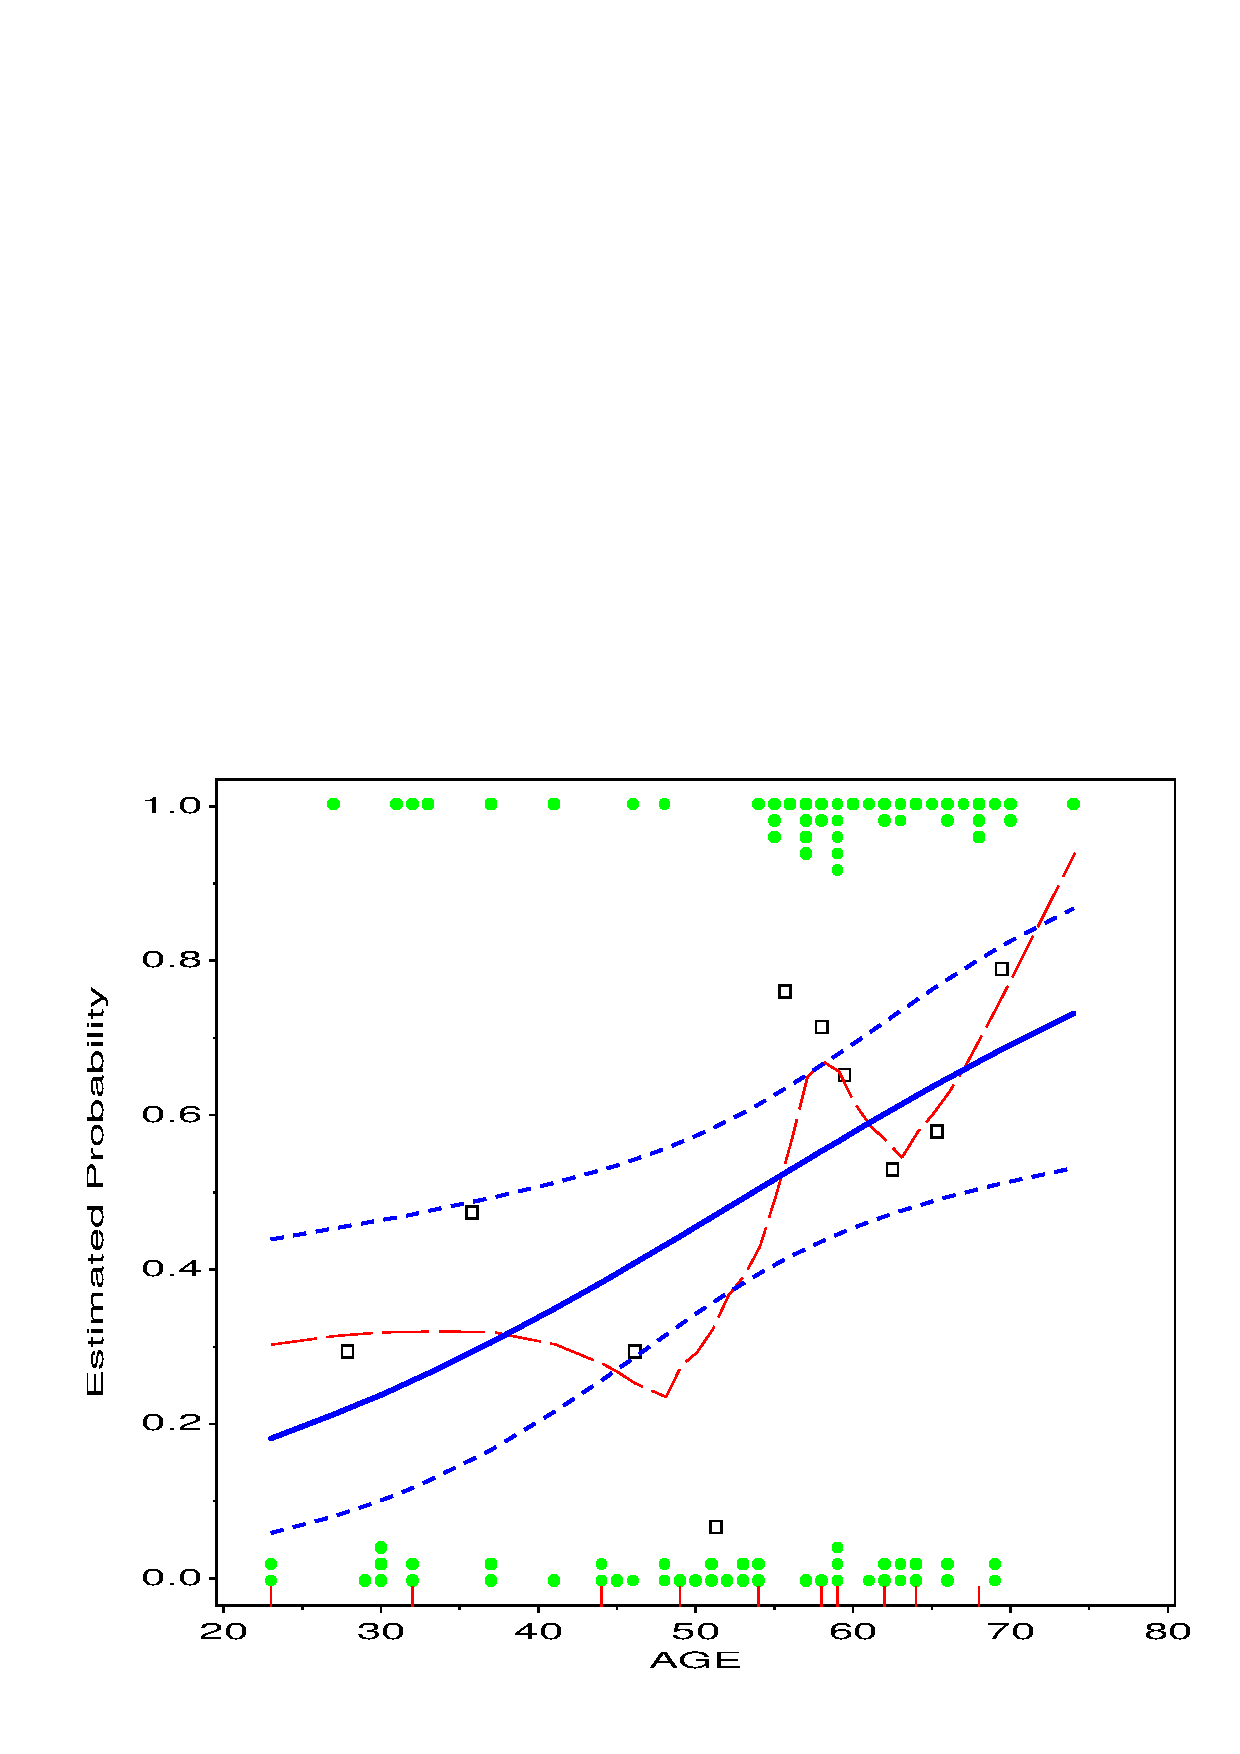
\includegraphics[width=1\linewidth]{ch6/fig/logoddt2}
 \end{minipage}
 \caption[Empirical log-odds and probability plots for arthritis treatment data]{Empirical log-odds and probability plots for arthritis treatment data.
 The observed responses are plotted as stacked points at the top and bottom of the figures.  The squares show the empirical sample logits, and the analogous adjusted sample probabilities.}\label{fig:logoddt}
\end{figure}

It is helpful, therefore, to plot the observed sample logits or
sample probabilities against $X$, together with the observations
(in a way which avoids overplotting), and the fitted relationships,
as we do in \figref{fig:logoddt}.
Suppose we group the observations into some number of intervals,
as in \tabref{tab:arthlogit},
and let $n_i$ denote the number of observations in the $i$th
interval, of which $y_i$ are successful events.

Then, the observed probability is $p_i = y_i / n_i$ in interval $i$,
and the sample logit is
$\log[ p_i / (1 - p_i) ] = \log[ y_i / (n_i - y_i)]$.
But as we saw in \tabref{tab:arthlogit}, the logit is not defined
when $y_i =0$, or when $y_i = n_i$.
We get around this difficulty by substituting the
\boldital{empirical logit},
\begin{equation*}
 \log \left( \frac{y_i + \frac12}{n_i - y_i + \frac12} \right)
 \comma
\end{equation*}
which is also a less biased estimator of the true logit.  Analogously, in
a plot of probabilities against $X$, we use the adjusted value
$ (y_i + \frac12) / (n_i - y_i + \frac12)$.

An alternative to grouping the observations into fixed intervals is to
imagine a sliding window, wide enough to contain a given fraction,
$f$ of the points, moving from left to right across the plot.
At each position of the window,  calculate a smoothed, locally weighted
average of the binary $y$ values within the window using the
\glossterm{lowess} scatterplot smoothing algorithm
\citep{Cleveland:79} (without robustness iterations).
This gives a smooth, nonparametric regression for $\hat{p}_i$,
advocated by \citet{Landwehr-etal:84} and \citet{Fowlkes:87}.
\citet{Copas:83} discusses methods based on kernel density estimation
for smoothing binary data.

These plots are produced by the \macro{LOGODDS}, documented in
\macref{mac:logodds}.
Both plots in \figref{fig:logoddt}
were produced by these statements:
\begin{listing}
%include data(arthrit);
data arthrit;
   set arthrit;
   format better outcome.;
%logodds(data=arthrit, x=age, y=Better, ncat=10, smooth=0.5);
\end{listing}

The macro assumes a quantitative predictor and groups the observations
into the number of intervals specified by the \mparm{NCAT=}{LOGODDS}.
The lower limits of the intervals are shown by the short vertical lines
above the horizontal axis.
When the \mparm{SMOOTH=}{LOGODDS}  is specified, the \macro{LOWESS}
\citep[App. A1.9]{Friendly:91} using that value as the smoothing parameter,
$f$, and the smoothed nonparametric curve is drawn on the probability
plot.
With moderate sample sizes, as we have here, the lowess curve may be quite
variable, and of course ignores other explanatory variables.

Note that the fitted regression relation is linear on the scale of log odds
(cf. \eqref{eq:logit1})
but (slightly) non-linear on the scale of probabilities
(cf. \eqref{eq:logit3}).
Because most people find it easier to interpret probabilities than log odds,
it is often useful to make a single plot showing \emph{both} scales.
